\section{Introducción}
\label{sec:intro}

El juego \emph{Sudoku} es un rompecabezas lógico que trata la ubicación de
números en una grilla de $9 x 9$. Este tiene celdas con valores ya fijados,
llamados \textit{pistas}, y el objetivo es completar las celdas
faltantes con dígitos del 1 al 9. La grilla se subdivide en $9$ cuadrantes de
$3 x 3$  que se debe completar cumpliendo con las siguientes reglas:

\begin{enumerate}
    \label{enum:principios}

    \item Cada fila debe tener los valores de 1 a 9 una única vez
    \item Cada columna debe tener los valores de 1 a 9 una única vez
    \item Cada subcuadrante de $3x3$ debe tener los valores de 1 a 9 una única vez
\end{enumerate}

Un ejemplo de este tipo de problemas tan conocido se observa en la figura \ref{img:sudoku}


\begin{figure}[H]
	\centering
	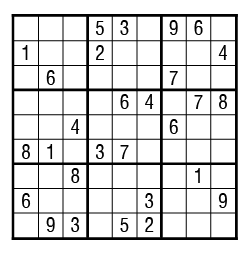
\includegraphics[scale=0.6]{./img/sudoku_ejemplo.png}
	\caption{Sudoku ejemplo}
	\label{img:sudoku}
\end{figure}


Dado que es un problema NP-Completo \cite{complexity}, durante los últimos tiempos, han surgido
diversos métodos para resolver de manera heurística el problema dada su complejidad.

Los métodos de resolución exacta para este problema con \emph{Fuerza bruta}
consisten en asignar posibles valores iterativamente a las celdas e ir
verificando si el Sudoku cumple las reglas a medida que se siguen completando
los blancos. Este algoritmo de resolución es costoso y a menudo se utiliza con backtracking. 
Se probo que existen aproximadamente $6.67 x 10^2^1$ grillas válidas posibles. 

En la actualidad se han encontrado avances en la resolución de Sudoku utilizando
algoritmos genéticos \cite{genetic}, Búsqueda armónica
\cite{harmony} y Colonia de hormigas \cite{ant_colony_1} entre otros.

Para este trabajo práctico, implementamos una metaheurística de Colonia de hormigas.
